\chapter{Experimenten en Resultaten}
\label{hoofdstuk:ER}
In dit hoofdstuk worden de belangrijkste experimenten besproken die uitgevoerd in het verloop van deze masterproef. Deze hebben zowel betrekking op de besproken melodische transformaties, de algoritmes om deze transformaties te combineren en ook het RPK-model dat gebruikt werd om deze transformaties te evalueren.\\
De resultaten worden meestal weergegeven op een plot waarbij op de y as de gemiddelde probabiliteit staat. Deze probabiliteit staat voor de gemiddelde probabiliteit van voorkomen van een noot (gegeven de vorige noot) volgens het RPK-model in alle muziekstukken waarop er getest werd. Als er dus in dit hoofdstuk gesproken wordt over een gemiddelde probabiliteit van een bepaald muziekstuk dan betekent dit de gemiddelde probabiliteit van een noot in dit muziekstuk.

\section{Vergelijking van de twee melodische transformaties}
\label{experiment:5}
\subsection{Beschrijving experiment}
Dit experiment heeft als opzet om de twee verschillende soorten transformaties die besproken werden in hoofdstuk \ref{hoofdstuk:MT} te vergelijken in performantie. De eerste transformatie gaat een noot in de melodielijn transformeren naargelang zijn positie in de notensequentie (deze transformatie noemen we in het vervolg van die onderdeel T1). De tweede transformatie gaat een noot transformeren enkel op basis van zijn (melodische) afstand ten opzichte van de vorige noot in de melodielijn (deze transformatie noemen we in de rest van dit onderdeel T2). De werking van deze twee transformaties staat beschreven respectievelijk in hoofdstukken \ref{MT:positie} en \ref{MT:afstand_vorige}.

Voor dit experiment zullen voor 50 testgevallen telkens 10 verschillende willekeurige voorkomens voor beide transformatie getest worden. Zo een willekeurige transformatie wordt bekomen door 8 opeenvolgende getallen tussen -5 en +6 (beide grenzen inclusief) willekeurig te genereren. Noem deze 8 getallen in volgorde $X_{i}$ met 0$\leq$ i$\leq$ 7. Voor T1 levert dit dan de transformatie op beschreven in tabel \ref{tabel:exp5:T1}, voor T2 levert dit de transformatie beschreven in tabel \ref{tabel:exp5:T2}.

\begin{table}
  \centering
  \begin{tabular}{c | c c c c c c c c }
    Pos (mod 8) & 0 & 1 & 2 & 3 & 4 & 5 & 6 & 7 \\
    \hline
    \hline
    Verhoging & $X_{0}$ & $X_{1}$ & $X_{2}$ & $X_{3}$ & $X_{4}$ & $X_{5}$ & $X_{6}$ & $X_{7}$ \\
  \end{tabular}
  \caption{Willekeurige transformatie volgens T1, gebruikt in het experiment van onderdeel \ref{experiment:5}.}
  \label{tabel:exp5:T1}
\end{table}

\begin{table}
  \centering
  \begin{tabular}{c | c c c c c c c c }
    Diff (mod 8) & 0 & 1 & 2 & 3 & 4 & 5 & 6 & 7 \\
    \hline
    \hline
    Verhoging & $X_{0}$ & $X_{1}$ & $X_{2}$ & $X_{3}$ & $X_{4}$ & $X_{5}$ & $X_{6}$ & $X_{7}$ \\
  \end{tabular}
  \caption{Willekeurige transformatie volgens T2, gebruikt in het experiment van onderdeel \ref{experiment:5}.}
  \label{tabel:exp5:T2}
\end{table}

Voor elk van de 50 testgevallen worden zo dus 20 transformaties gegenereerd (10 voor T1 en 10 voor T2). Over deze 50 testgevallen en 10 transformaties per transformatie soort wordt dan een gemiddelde consonantiescore berekend. De exponenti\"ele van deze consonantie score levert dan voor beide transformatie soorten een gemiddelde probabiliteit van een getransformeerd muziekstuk.

\subsection{Resultaten}

\begin{table}
  \centering
  \begin{tabular}{c | c c }    
    Transformatie & Consonantiescore & Probabiliteit(\%)\\
    \hline
    Oiginele melodie & -2.36 & 9.42\\
    T1 & -3.72 & 2.43\\
    T2 & -3.19 & 4.12\\
  \end{tabular}
  \caption{Resulaten van experiment \ref{experiment:5}. Gemiddelde consonantiescores voor de twee soorten transformaties en de originele melodielijnen die getranformeerd werden. De twee geteste soorten van transformaties staan beschreven in onderdelen \ref{MT:positie}(T1) en \ref{MT:afstand_vorige}(T2).}
  \label{tabel:res5}
\end{table}

In tabel \ref{tabel:res5} staan de resultaten van dit experiment weergegeven. Er valt meteen op dat beide transformaties de originele melodielijnen gemiddeld gezien transformeren naar een nieuwe melodielijn met een minder goede consonantiescore. Er is ook een duidelijk verschil merkbaar in kwaliteit van de transformaties, T2 scoort merkbaar beter dan T1. Dit is ook logisch aangezien T1 eigenlijk niets van informatie over het muziekstuk in rekening brengt, buiten zijn absolute positie (modulo 8). T2 brengt de afstand tot de vorige noot in rekening wat er toe kan leiden dat in sommige gevallen de intervallen tussen opeenvolgende noten relatief kleiner gehouden wordt dan bij T1, wat consistenter betere scores kan opleveren volgens het RPK-model.

\section{Vergelijking Fibonacci transformatie met gemiddelde transformatie}
\label{experiment:6}
\subsection{Beschrijving experiment}
Het doel van dit experiment is om na te gaan of een transformatie, die gebaseerd is op de rij van Fibonacci een beter resultaat geeft dan een gemiddelde transformatie. De reden dat er specifiek getest wordt op de rij van Fibonacci is omdat deze bekende rij in zoveel verschillende onderdelen van de natuur te herkennen valt dat het in zeker zin niet onlogisch zou zijn, moest deze ook in de muziek onder bepaalde vormen voorkomen. Voor beide soorten van transformaties die beschreven staan in onderdelen \ref{MT:positie} en \ref{MT:afstand_vorige} (en die we in het kort respectievelijk T1 en T2 noemen), wordt zo een transformatie gecre\"eerd die gebaseerd is op de rij van fibonacci. Deze transformaties worden beschreven door tabellen \ref{tabel:exp6:T1} en \ref{tabel:exp6:T2}. Hierbij is elk getal op de onderste rij telkens de gelijk aan het overeenkomstig element uit de rij van fibonacci modulo 12, waarbij de waarde van elke sprong tussen -5 en +6 ligt.

\begin{table}
  \centering
  \begin{tabular}{c | c c c c c c c c }
    Positie (mod 8) & 0 & 1 & 2 & 3 & 4 & 5 & 6 & 7 \\
    \hline
    \hline
    Verhoging & 1 & 1 & 2 & 3 & 5 & -4 & 1 & -3 \\
  \end{tabular}
  \caption{Fibonacci transformatie volgens T1 gebruikt in het experiment van onderdeel \ref{experiment:6}.}
  \label{tabel:exp6:T1}
\end{table}

\begin{table}
  \centering
  \begin{tabular}{c | c c c c c c c c }
    Diff (mod 8) & 0 & 1 & 2 & 3 & 4 & 5 & 6 & 7 \\
    \hline
    \hline
    Verhoging & 1 & 1 & 2 & 3 & 5 & -4 & 1 & -3 \\
  \end{tabular}
  \caption{Fibonacci transformatie volgens T2 gebruikt in het experiment van onderdeel \ref{experiment:6}.}
  \label{tabel:exp6:T2}
\end{table}

Nu wordt op dezelfde 50 testgevallen als waarop getest werd in experiment \ref{experiment:5}, deze twee transformaties toegepast. De gemiddelde consonantiescores die deze twee Fibonacci transformaties opleveren kunnen nu vergeleken worden met het gemiddelde algemene geval voor de twee soorten transformaties. 

\subsection{Resultaten}

\begin{table}
  \centering
  \begin{tabular}{c | c c }    
    Transformatie & Consonantiescore & Probabiliteit(\%)\\
    \hline
    Oiginele melodie & -2.36 & 9.42\\
    T1 & -2.92 & 5.42\\
    T2 & -2.63 & 7.21\\
  \end{tabular}
  \caption{Resulaten van experiment \ref{experiment:6}. Gemiddelde consonantiescores voor de twee Fibonacci transformaties en de originele melodielijnen die getranformeerd werden.}
  \label{tabel:res6}
\end{table}

Tabel \ref{tabel:res6} geeft de resultaten van de Fibonacci transformaties weer. In tabel \ref{tabel:res5} staan de resultaten van dezelfde soorten transformaties maar dan met willekeurige sprongen in plaats van sprongen volgens de rij van Fibonacci. Er valt op dat voor beide transformatie soorten, de transformatie volgens de rij van Fibonacci merkbaar beter scoort dan een gemiddelde transformatie van zijn soort. Een reden hiervoor is dat de sprongen in de Fibonacci transformaties redelijk klein zijn (bijvoorbeeld drie keer op acht een sprong van slechts een halve toon). Hierdoor zal het originele muziekstuk minder aangepast worden en de score dus ook niet zo veel verslechteren dan na een gemiddelde transformatie. 

Voor de Fibonacci transformatie volgens T2 kan zelfs gezegd worden dat deze zeer goed scoort, aangezien de consonantiescore die gemiddeld bekomen wordt met deze transformatie zelfs in de buurt ligt van de originele melodielijn. De reden hiervoor is dat er bij deze transformatie veel dezelfde noten na elkaar gecre\"eerd worden (wat goede scores geeft voor het RPK-model aangezien de \textit{proximity} maximaal is). Dit komt doordat sprongen in dit algoritme in tegengestelde richting uitgevoerd worden als de afstand ten opzichte van de vorige noot. En afstanden van grootte 1, 2 en 3 worden bijvoorbeeld allemaal gecounterd door een sprong van dezelfde grootte in tegengestelde richting. Hierdoor zullen noten die op zo een afstand van elkaar zitten telkens op dezelfde noot afgebeeld worden.

Er kan dus besloten worden dat deze Fibonacci transformaties iets betere resultaten leveren dan een gemiddelde transformatie (wat de consonantiescore betreft). Dit betekent echter niet automatisch dat de muziekstukken ook beter klinken want bijvoorbeeld bij de Fibonacci transformatie volgens tabel \ref{tabel:exp6:T2} zullen sequenties gecre\"eerd worden die veel dezelfde noten bevatten, wat over het algemeen niet als interessante muziek beschouwd wordt.

\section{Transformaties combineren: 1 transformatie, meerdere iteraties}
\label{experiment:1}
\subsection{Beschrijving experiment}
Dit experiment heeft betrekking tot het algoritme dat besproken werd in onderdeel \ref{ETT:algo1}. Dit experiment gaat nagaan wat de invloed is van het aantal iteraties van het aantal iteraties van dit algoritme op de consonantiescore van het totale muziekstuk. Er wordt in dit algoritme slechts gebruik gemaakt van een transformatie. Deze gebruikte transformatie wordt weergegeven in tabel \ref{tabel:exp1}.

\begin{table}
  \centering
  \begin{tabular}{c | c c c c c c c c }
    Diff (mod 8) & 0 & 1 & 2 & 3 & 4 & 5 & 6 & 7 \\
    \hline
    \hline
    Verhoging & 5 & -4 & 1 & -3 & 1 & 1 & 2 & 3 \\
  \end{tabular}
  \caption{Transformatie gebruikt in het experiment van onderdeel \ref{experiment:1}.}
  \label{tabel:exp1}
\end{table}

Deze test wordt uitgevoerd op 100 muziekstukken uit het Essencorpus. De gemiddelde probabiliteit van de originele stukken wordt berekend alsook de gemiddelde probabiliteit van het muziekstuk dat optimaal is volgens het RPK-model in de toonaard van de 100 stukken. Nu kan er gekeken worden naar hoe snel de consonantiescore zich gaat verplaatsten van die van het originele naar die van de theoretisch best mogelijke volgens het model afhankelijk van het aantal iteraties dat het algoritme wordt uitgevoerd.

\subsection{Resultaten}

\begin{figure}[!ht]
  \centering
  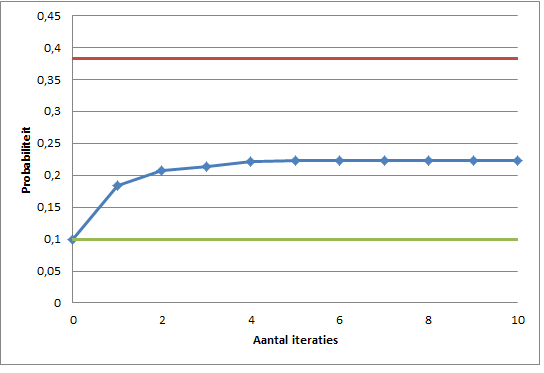
\includegraphics[width=0.75\textwidth]{5_Experimenten_Resultaten/exp1_res}
  \caption{Resultaten van het experiment uitgevoerd in deel \ref{experiment:1}. De groene lijn staat voor de gemiddelde probabiliteit van een noot in de originele melodie, de rode lijn voor de gemiddelde probabiliteit van de theoritisch beste melodielijn in de toonaarden waarop getest werd en de blauwe lijn geeft de gemiddelde probabiliteit van een noot weer na uitvoer van het algoritme na een verschillend aantal iteraties.}
  \label{figuur:exp1}
\end{figure}

In figuur \ref{figuur:exp1} worden de restultaten weergegeven van dit experiment. De groene lijn op de figuur geeft de gemiddelde probabiliteit weer van alle melodie\"en waarop getest werd. De rode lijn geeft voor al deze melodie\"en de gemiddelde waarde mee voor het theoretisch beste muziekstuk dat volgens het RPK-model gemaakt kan worden in deze toonaard. Tot slot geeft de blauwe lijn de gemiddelde probabiliteit weer van een noot in de getransformeerde melodie, na toepassing van 1 tot 10 iteraties van de transformatie.\\
Er valt duidelijk op dat de eerste paar iteraties nog een redelijke verhoging van de probabiliteit teweeg brengt, maar dat na een vijftal iteraties gemiddeld gezien een soort van maximum bereikt is dat met deze transformatie kan bekomen worden. De reden dat deze waarde nog zo ver onder het theoretische maximum ligt, heeft er vooral mee te maken dat er maar 1 mogelijke transformatie is dat het algoritme mag gebruiken, hierdoor zijn er nog steeds maar een zeer beperkt aantal mogelijkheiden om een bepaalde noot te transformeren, en kunnen bijgevolg nog steeds de meeste noten niet bereikt worden vanuit eender welke noot.

\section{Transformaties combineren: meerdere transformaties, 1 iteratie}
\label{experiment:2}
\subsection{Beschrijving experiment}
Dit experiment heeft betrekking tot het algoritme dat besproken werd in onderdeel \ref{ETT:algo1}. Het experiment gaat nagaan wat de invloed is van het aantal verschillende toegelaten transformaties op de consonantiescore van het totale muziekstuk. Zo zijn de vijf transformaties die gebruikt zullen worden weergegeven in tabel \ref{tabel:exp2}. Er wordt nu telkens slechts een iteratie van het algoritme uitgevoerd.\\

\begin{table}
  \centering
  \begin{tabular}{c | c c c c c c c c }
    Diff (mod 8) & 0 & 1 & 2 & 3 & 4 & 5 & 6 & 7 \\
    \hline
    \hline
    Verhoging transformatie 1 & 5 & -4 & 1 & -3 & 1 & 1 & 2 & 3 \\
    \hline
    Verhoging transformatie 2 & 1 & 3 & 4 & -5 & -1 & 6 & 5 & -1 \\
    \hline
    Verhoging transformatie 3 & 1 & 4 & 5 & -3 & 2 & -1 & 1 & 0 \\
    \hline
    Verhoging transformatie 2 & 4 & 6 & -2 & 4 & 2 & 6 & -4 & 2 \\
    \hline
    Verhoging transformatie -2 & -3 & -2 & 3 & -1 & 4 & -3 & 2 & -4 \\
  \end{tabular}
  \caption{Transformaties gebruikt in het experiment van onderdeel \ref{experiment:2}.}
  \label{tabel:exp2}
\end{table}

Deze test wordt uitgevoerd op 50 muziekstukken uit het Essencorpus. De gemiddelde probabiliteit van de originele stukken wordt berekend alsook de gemiddelde probabiliteit van het muziekstuk dat optimaal is volgens het RPK-model in de toonaard van de 50 stukken. Nu kan er weer gekeken worden naar hoe snel de consonantiescore zich gaat verplaatsten van die van het originele naar die van de theoretisch best mogelijke volgens het model afhankelijk van het aantal transformaties dat aan het algoritme ter beschikking wordt gesteld. Het experiment wordt eerst uitgevoerd met slechts een mogelijke transformatie. Dit zal dan transformatie 1 uit de tabel zijn. Daarna wordt het experiment uitgevoerd met 2 mogelijke transformaties. Dit zullen dan de eerste twee transformaties uit de tabel zijn enz..

\subsection{Resultaten}

\begin{figure}[!ht]
  \centering
  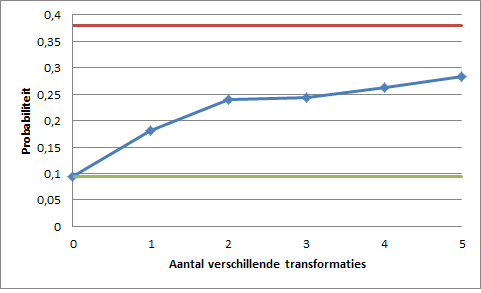
\includegraphics[width=0.75\textwidth]{5_Experimenten_Resultaten/exp2_res}
  \caption{Resultaten van het experiment uitgevoerd in deel \ref{experiment:2}. De groene lijn staat voor de gemiddelde probabiliteit van een noot in de originele melodie, de rode lijn voor de gemiddelde probabiliteit van de theoritisch beste melodielijn in de toonaarden waarop getest werd en de blauwe lijn geeft de gemiddelde probabiliteit van een noot weer na uitvoer van het algoritme afhankelijk van het aantal transformaties dat ter beschikking gesteld was aan het algoritme.}
  \label{figuur:exp2}
\end{figure}

In figuur \ref{figuur:exp2} worden de restultaten weergegeven van dit experiment. Het is duidelijk dat een  hoger aantal transformaties ook telkens een betere score teruggeeft. Als we de resultaten van dit experiment vergelijken met dat uit onderdeel \ref{experiment:1}, dan merken we op dat het aantal transformaties een grotere impact heeft op de probabiliteit dan het aantal iteraties. De grootste reden hiervoor is dat een extra transformaties er voor kan zorgen dat er voor elke een noot in het muziekstuk een extra mogelijke noot is waarnaar hij getransformeerd kan worden. Dit zorgt voor enorm veel extra mogelijkheden waardoor er hogere probabiliteiten kunnen bekomen worden dan in het geval waarbij het aantal iteraties verhoogd wordt in plaats van het aantal mogelijke transformaties.  


\section{Transformaties combineren: minimum transformatie lengte}
\label{experiment:3}
\subsection{Beschrijving experiment}
Dit experiment heeft betrekking tot het algoritme dat besproken werd in onderdeel \ref{ETT:algo2}. Het experiment gaat nagaan wat de invloed is van de minimum transformatielengte op de consonantiescore van het totale muziekstuk. Er wordt in dit experiment telkens gebruik gemaakt van 2 transformaties die beschreven zijn in tabel \ref{tabel:exp3}. Er wordt telkens slechts een iteratie van het algoritme uitgevoerd.\\

\begin{table}
  \centering
  \begin{tabular}{c | c c c c c c c c }
    Diff (mod 8) & 0 & 1 & 2 & 3 & 4 & 5 & 6 & 7 \\
    \hline
    \hline
    Verhoging transformatie 1 & 5 & -4 & 1 & -3 & 1 & 1 & 2 & 3 \\
    \hline
    Verhoging transformatie 2 & 1 & 3 & 4 & -5 & -1 & 6 & 5 & -1 \\
  \end{tabular}
  \caption{Transformaties gebruikt in het experiment van onderdeel \ref{experiment:3}.}
  \label{tabel:exp3}
\end{table}

Dit experiment wordt uitgevoerd op 50 muziekstukken uit het Essencorpus en dit voor alle waarden van de minimum transformatie lengte tussen 1 en 10. Voor elk van deze 10 gevallen wordt de gemiddelde probabiliteit van het getransformeerde muziekstuk berekend.

\subsection{Resultaten}

\begin{figure}[!ht]
  \centering
  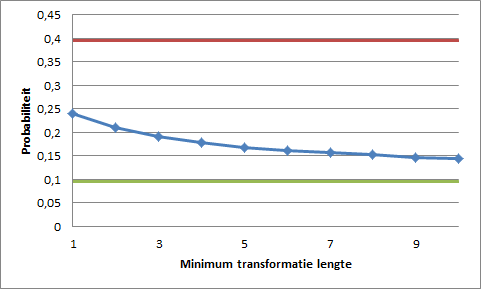
\includegraphics[width=0.75\textwidth]{5_Experimenten_Resultaten/exp3_res}
  \caption{Resultaten van het experiment uitgevoerd in deel \ref{experiment:3}. De groene lijn staat voor de gemiddelde probabiliteit van een noot in de originele melodie, de rode lijn voor de gemiddelde probabiliteit van de theoritisch beste melodielijn in de toonaarden waarop getest werd en de blauwe lijn geeft de gemiddelde probabiliteit van een noot weer na uitvoer van het algoritme afhankelijk van de minimum transformatie lengte.}
  \label{figuur:exp3}
\end{figure}

Figuur \ref{figuur:exp3} geeft de resultaten weer van het experiment. Het is duidelijk dat een hogere minimum transformatie lengte leidt tot een kleinere verbetering van de consonantiescore, wat te verwachten was. De grafiek is ook monotoon dalen voor stijgende waarde van de minimum transformatie lengte. Dit moet ook zo zijn aangezien alle transformaties die geldig zijn voor een zekere transformatie lengte ook altijd geldig zijn voor alle kortere transformatie lengtes.

\section{Transformaties combineren: Gelijkheid algoritmen voor transformatie lengte 1}
\label{experiment:4}
\subsection{Beschrijving experiment}
Dit experiment is opgezet als extra test om het geloof in de juiste werking van de algoritmes beschreven in \ref{ETT:algo1} en \ref{ETT:algo2} te versterken. Aangezien de implementaties van deze twee algoritmen toch op een aantal vlakken (vooral de voorstelling van de paden) verschillen van elkaar, is het interessant om voor een minimum transformatie lengte van 1 eens te kijken of de twee algoritmes hetzelfde resultaat geven. Dit zou normaal gezien altijd het geval moeten zijn aangezien de twee algoritmes hetzelfde doel en dezelfde middelen hebben in het geval van een minimum transformatie lengte van 1. De transformatie waarvan gebruik gaat worden gemaakt staat beschreven in tabel \ref{tabel:exp4}.

\begin{table}
  \centering
  \begin{tabular}{c | c c c c c c c c }
    Diff (mod 8) & 0 & 1 & 2 & 3 & 4 & 5 & 6 & 7 \\
    \hline
    \hline
    Verhoging & 5 & -4 & 1 & -3 & 1 & 1 & 2 & 3 \\
  \end{tabular}
  \caption{Transformatie gebruikt in het experiment van onderdeel \ref{experiment:4}.}
  \label{tabel:exp4}
\end{table}

Voor deze transformatie gaat het experiment zoals het beschreven staat in onderdel \ref{experiment:1} herhaald worden maar dan ook voor het tweede algoritme. Dus voor een aantal iteraties van 1 tot en met 10 van het algoritme gaan de probabiliteiten die beide algoritmes opleveren voor dezelfde transformatie op dezelfde 100 testgevallen uit het Essencorpus vergeleken worden.

\subsection{Resultaten}

\begin{table}
  \centering
  \begin{tabular}{c | c | c }    
    \# iteraties & Algoritme 1 & Algoritme 2 \\
    \hline
    1 & -1.69 & -1.69\\
    2 & -1.57 & -1.57\\
    3 & -1.54 & -1.54\\
    4 & -1.51 & -1.51\\
    5 & -1.50 & -1.50\\
    6 & -1.50 & -1.50\\
    7 & -1.50 & -1.50\\
    8 & -1.50 & -1.50\\
    9 & -1.50 & -1.50\\
    10 & -1.50 & -1.50\\
  \end{tabular}
  \caption{Resulaten van experiment \ref{experiment:4}. Gemiddelde consonantiescores voor de twee algoritmen (logaritme van de probabiliteit) na een gegeven aantal iteraties. Algoritme 1 staat beschreven in \ref{ETT:algo1}, algoritme 2 is hetgene dat beschreven staat in \ref{ETT:algo2}.}
  \label{tabel:res4}
\end{table}

In tabel \ref{tabel:res4} staan de resultaten van dit experiment weergegeven. Beide algoritmen leveren dezelfde gemiddelde consonantiescore (logaritme van de gemiddelde probabiliteit) voor een muziekstukje na eenzelfde aantal iteraties gebruik makende van dezelfde transformatie. Dit versterkt de stelling dat de twee algoritmes wel degelijk werken zoals gewenst.

\section{Test Performantie algoritmes}
\label{experiment:7}
\subsection{Beschrijving experiment}

\subsection{Resultaten}

%%% Local Variables: 
%%% mode: latex
%%% TeX-master: "masterproef"
%%% End: 
